% 中文版：单栏排版，由 paper-new/acl/main.tex 翻译而来。
% 编译：xelatex zh_main -> bibtex zh_main -> xelatex zh_main x2
\documentclass[12pt,a4paper]{article}
\usepackage{ctex}
\usepackage[margin=2.5cm]{geometry}
\usepackage{amsmath,amssymb,booktabs,graphicx,multirow,float}
\usepackage[authoryear]{natbib}
\usepackage[hidelinks]{hyperref}
\usepackage{caption}
\usepackage{tikz}
\usetikzlibrary{arrows.meta, positioning, fit, calc, backgrounds}
\definecolor{oiBlue}{RGB}{0,114,178}
\definecolor{oiOrange}{RGB}{213,94,0}
\definecolor{oiGreen}{RGB}{0,158,115}
\definecolor{oiGray}{RGB}{110,110,110}
\captionsetup{font=small,labelsep=quad}
\setlength{\parskip}{2pt}
\graphicspath{{../figures/}}


\title{TRACER：面向递归序列模型的词元级分析、计算控制与进化式潜状态精化}
\author{匿名作者}

\begin{document}
\maketitle

\begin{abstract}
递归序列模型通过反复执行共享的精化算子改善预测，但多数部署对每个词元执行相同数量的步骤。这把计算花在已经正确的词元上。三个问题仍未解决：额外步骤是否真的被执行、潜状态内部发生了什么、步长策略能否迁移。我们发现高置信词元在不同深度下保持预测不变，其精化因此冗余，也为提前停止提供了依据。我们提出 TRACER，一个测量词元级转移、基于因果置信度停算、审计实际执行调用并在固定预算下搜索潜状态步长的框架。在 TRACER 中，一次性的 3{,}000 样本 COGS 开发集检查显示，冻结 GRU 上的阈值停算在两个种子上执行最深基准 25.7\% 的调用，在第三个种子上执行较浅 $e_1$ 基准 51.8\% 的调用，精确匹配变化不超过 0.20pp。执行钩子确认被跳过的精化不触发任何调用。潜状态轨迹显示，有界门控态在第一次精化后饱和，而无界累积态持续增长。跨四个架构，12 个种子中 9 个非劣或更优，2 个显著更差。45 次搜索的中位增益为 0.52pp，即 192 样本内层子集中的一个样本；冻结在 GRU 上的策略在 9 个目标种子中的 4 个上非劣，无一显著更差。我们公开框架与审计协议。
\end{abstract}

\section{引言}
\label{sec:intro}

递归序列模型复用共享的精化单元，使早期错误能在后续步骤中被修复，而无需增加参数。把 Transformer 写成循环更新使这一视角具有普适性 \citep{katharopoulos2020transformers}，循环 Transformer 的研究表明，重复同一计算可以实现单遍无法完成的计算 \citep{giannou2023looped,yang2024looped}。早期的多跳与关系循环也说明了同一点 \citep{sukhbaatar2015memory,santoro2018relational}。Universal Transformer 与递归 GRU 的研究表明，这类额外计算能改善推理与语义解析 \citep{dehghani2019universal,graves2016adaptive}。标准部署预先固定遍数，让每个词元经过相同深度，即使条件计算与词元级路由允许模型在不同输入上花费不同计算 \citep{fedus2022switch,raposo2024mixture}。词元难度不同：许多词元在第一遍后已经正确，少数才需要额外步骤。在 COGS \citep{kim2020cogs} 上，一个组合泛化仍然困难的基准 \citep{lake2018generalization,oren2020improving}，87\%--91\% 的样本在第一次精化前后保持预测不变，只有 5\%--9\% 被修复。问题在于，预测已经稳定的词元是否还需要剩余的精化步骤。

固定深度下的准确率很少说明产生它的计算过程。相邻深度只在少数词元上改变预测，后续步骤甚至可能把一个正确答案翻转，这种失败被称为过度思考 \citep{kaya2019shallowdeep}。这一差异无法告诉我们模型是存入了新信息，还是仅仅重写了同一状态。低维轨迹、不动点与更新方向是描述循环动力学的常用词汇 \citep{sussillo2013blackbox,vyas2020population,haviv2019memory}，表示相似性分析则提醒我们，不同系统的绝对坐标不可直接比较 \citep{kriegeskorte2008rsa,kornblith2019cka}。为此，我们在四个架构的每个深度记录潜状态，比较其范数、位移、方向与预测变化。在有界状态模型中，第一次精化贡献了大部分状态变化，后续更新收缩为其中一小部分，且这一模式只在深度一后准确率已饱和的种子上成立。无界状态的表现不同：Transformer 的更新在各深度几乎共线，状态范数随深度稳步增长。这一对比引出关于更新规则本身的第二个问题。在潜空间中做迭代精化可以在恒定计算下改变结果 \citep{lee2020iterative,geng2021rewrite}，因此固定的精化规则未必最好。可以在固定评估预算下搜索一个低维步长，而进化方法长期用于在不穿过网络反向传播的情况下搜索控制器参数 \citep{stanley2002neat,such2017neuro}。冻结在一个模型上的策略能否在另一个模型上继续成立，则是另一个待检验的经验问题。

我们提出 TRACER，一个把递归视为先测量、再控制的对象的框架。第一个组件仅使用其所门控的精化之前就已可得的置信度停算词元；基于置信度的推理早已用这类读数调整深度或弃答 \citep{liu2020fastbert,xin2020deebert,geifman2017selective}。带前向钩子的 active-subset 执行器确认被跳过的精化确实没有被计算。第二个组件记录四个架构的潜状态轨迹，把每条轨迹化为范数、位移与更新方向；这些摘要描述模型内部跨精化的变化，揭示首次增益在何处饱和、何处没有。第三个组件在 336 次评估的等预算下搜索一个五参数步长策略，并在留出数据与三个未见架构上检验冻结后的策略。等预算比较很重要，因为增益相对于种子波动很小，而非劣效检验为"以更少计算换取不损失准确率"提供了合适的统计框架 \citep{docampobayon2025noninferiority,gu2023evaluation}。在 COGS 上，停算在多数种子上以最深调用数的四分之一保持准确率，审计过的执行器确认节省的调用并未执行，单序列延迟随调用数下降。跨架构轨迹呈现两种状态机制，而非一种普适的精化动力学。进化搜索的中位增益为内层子集的一个样本，冻结策略只在部分目标种子上非劣。我们与正面结果一并报告这些边界。



\section{相关工作}
\label{sec:related}

复用共享计算核心的循环计算有很长的历史。神经程序解释器让核心调用子程序并可终止 \citep{reed2016programmer}，神经图灵机则用有限控制器配以外接记忆 \citep{graves2014neural}。端到端记忆网络在多个跳上重复同一注意力模块 \citep{sukhbaatar2015memory}，关系循环网络在点积注意力中增强循环状态 \citep{santoro2018relational}。Transformer-XL 把状态跨段传递 \citep{dai2019transformerxl}，循环记忆 Transformer 引入显式记忆词元 \citep{bulatov2022recurrent}，RWKV 把线性注意力改写为循环更新 \citep{peng2023rwkv}。Retentive 网络把循环与注意力连接为三种等价的计算视角 \citep{sun2023retentive}。这些工作表明，重复计算能在参数不成比例增加的前提下改善预测。多数评估仍止于最终准确率：它们报告更深递归达成了什么，而不是每次精化贡献多少、多久改变一次决策，或潜状态是否真的发生变化。

动态深度从多个角度被研究过。BranchyNet 在中间层放置早退分类器 \citep{teerapittayanon2016branchynet}，多尺度密集网络让每一层都成为出口 \citep{huang2018multiscale}。空间自适应计算时间按图像位置分配层数 \citep{figurnov2017spatially}，这是词元级计算分配在视觉上的对应物。Bolukbasi 等人用全局目标学习逐层退出 \citep{bolukbasi2017adaptive}，FastBERT 与 DeeBERT 则把置信度门控退出用于预训练语言模型 \citep{liu2020fastbert,xin2020deebert}。基于预测稳定性的 patience 退出不只依赖单一概率 \citep{zhou2020patience}，mixture-of-depths 让不同词元经过不同层数 \citep{raposo2024mixture}，Switch Transformer 则通过每词元只激活部分参数来规模化条件计算 \citep{fedus2022switch}。这些方法把退出决策与网络联合训练，通常按控制器选出的深度或步数报告节省。冻结模型没有这样的门控可训练，阈值只能读取决策点已经存在的信号，而这些信号本身的质量也是被研究的问题 \citep{jiang2018trust,tian2023calibration}。节省是否真实，还要看解码器是否真的省略了被门控的精化，这需要数实际调用而不是推断深度。

迭代精化在多遍中修订初始输出。确定性非自回归建模把每一遍视为去噪步骤 \citep{lee2018deterministic}，潜空间精化把更新移到低维连续空间 \citep{lee2020iterative}。MR-P 让解码器在精化收敛时停止 \citep{cheng2022mrp}，近期的实证研究报告了精化步中的冗余改写与置信度变化 \citep{xiao2025empirical}。语义解析的工作表明，结构化改写能修复单遍遗漏的片段级错误 \citep{geng2021rewrite}。在这些工作中，遍数要么固定，要么由训练好的控制器选择；本文保持遍数固定，转而追问在冻结模型下每一步施加的更新能否被重新缩放。

轨迹读数为"一次精化改变了什么"提供了词汇。高维循环网络中的低维动力学用不动点与状态几何描述 \citep{sussillo2013blackbox,vyas2020population}，状态速度刻画一步内轨迹移动多远 \citep{haviv2019memory}。动力学相似性分析提醒我们，等价计算未必共享同一几何 \citep{ostrow2023dsa}，结构化状态空间模型定义的状态在尺度与含义上都不同于门控循环态 \citep{gu2022s4,gu2023mamba}。逐单元可视化说明了为何 LSTM 的细胞状态与隐状态必须分开读取 \citep{karpathy2015rnn}，几何研究则逐层分析表示动力学 \citep{horoi2020geometry}。这些观察支持在模型内对范数、位移与方向做摘要，也排除了用绝对状态范数给架构排名。

无导数搜索提供第三个组件。遗传算法仍是标准的黑盒优化器 \citep{whitley1994tutorial}，差分进化用种群成员间的差向量作为扰动 \citep{storn1997de,das2011survey}，CMA-ES 则依据搜索 landscape 自适应协方差矩阵 \citep{hansen2001cma,hansen2003cma}。无导数优化综述在统一的函数值预算下比较这些方法 \citep{rios2013df}，进化方法自 NEAT 起就被用于搜索网络拓扑与控制器 \citep{stanley2002neat,such2017neuro}。本文的搜索只调整已执行精化的步长，权重保持固定，各算法预算相同。我们要问的是，五参数更新策略在恒定深度下能带来多少增益，这份增益能否在留出数据上保留，又能否迁移到另一架构。

\section{方法}
\label{sec:method}

起点是一个冻结的递归序列模型，它给出从 $e_0$ 到 $e_3$ 四个解码深度。基步读取源端记忆、上一词元与上一隐状态，产生 $z^{(0)}$。共享的精化单元再用上一词元、基步的注意力上下文与当前预测的软嵌入，把 $z^{(k)}$ 映射为 $z^{(k+1)}$。下文所用的检查点在四个深度上都施加多深度监督，权重为 $(0.1,0.2,0.3,0.4)$，输出头在各深度共享。后续组件保持这些参数不变，都在同一条四深度展开上工作。

\begin{figure}[H]
\centering
\resizebox{\columnwidth}{!}{%
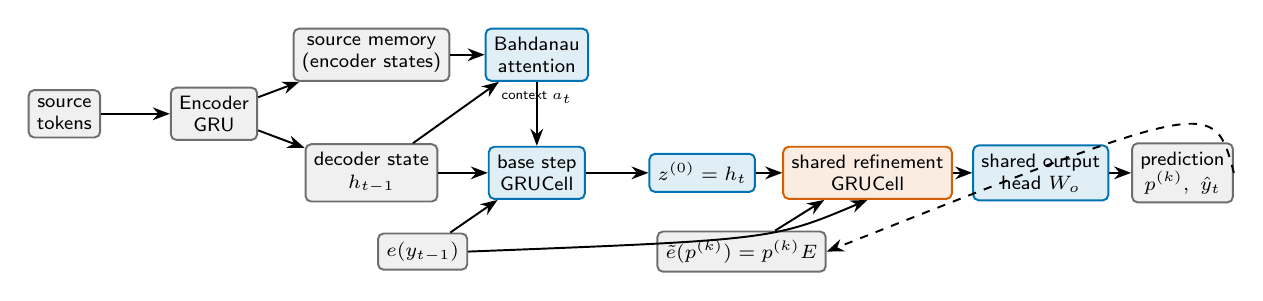
\begin{tikzpicture}[font=\sffamily\scriptsize, >=Stealth, line width=0.7pt,
  b/.style={draw, rounded corners=2pt, align=center, inner sep=3pt},
  g/.style={b, draw=oiGray, fill=oiGray!10},
  u/.style={b, draw=oiBlue, fill=oiBlue!12},
  o/.style={b, draw=oiOrange, fill=oiOrange!12}]
\node[g] (src) at (0,0) {source\\tokens};
\node[g] (enc) at (1.9,0) {Encoder\\GRU};
\node[g] (mem) at (3.9,0.75) {source memory\\(encoder states)};
\node[g] (st) at (3.9,-0.75) {decoder state\\$h_{t-1}$};
\node[u] (att) at (6.0,0.75) {Bahdanau\\attention};
\node[u] (base) at (6.0,-0.75) {base step\\GRUCell};
\node[g] (emb) at (4.55,-1.75) {$e(y_{t-1})$};
\node[u] (z0) at (8.1,-0.75) {$z^{(0)}=h_t$};
\node[o] (ref) at (10.2,-0.75) {shared refinement\\GRUCell};
\node[g] (soft) at (8.6,-1.75) {$\tilde e(p^{(k)})=p^{(k)}E$};
\node[u] (out) at (12.4,-0.75) {shared output\\head $W_o$};
\node[g] (pred) at (14.2,-0.75) {prediction\\$p^{(k)},\ \hat y_t$};
\draw[->] (src) -- (enc);
\draw[->] (enc) -- (mem); \draw[->] (enc) -- (st);
\draw[->] (mem) -- (att); \draw[->] (st) -- (att);
\draw[->] (att) -- node[above,font=\sffamily\tiny] {context $a_t$} (base);
\draw[->] (emb) -- (base); \draw[->] (st) -- (base);
\draw[->] (base) -- (z0); \draw[->] (z0) -- (ref);
\draw[->] (soft) -- (ref); \draw[->] (emb.east) .. controls (9.0,-1.6) .. (ref.south);
\draw[->] (ref) -- (out); \draw[->] (out) -- (pred);
\draw[->,dashed] (pred.east) .. controls (14.6,0.2) .. (soft.east);
\end{tikzpicture}%
}
\caption{递归编码器--解码器架构（依据实际实现绘制）。编码器产生源端记忆与初始解码状态；基步 	extsc{GRUCell} 由上一词元嵌入与注意力上下文得到 $z^{(0)}$。所有深度共享同一个精化 	extsc{GRUCell} 与同一个输出头，深度增加不引入新参数。}
\label{fig:arch}
\end{figure}

在这条展开上，先看额外深度带来了什么。对每个词元，比较相邻两个深度的预测，归入四类结果之一。错误预测变正确是修复，正确变错误是损害。预测未变时，原本正确记为保持，原本错误记为未解决。这种区分很必要：单一深度的准确率把被精化修复的词元与被精化破坏的词元算在一起。

\begin{figure}[H]
\centering
\resizebox{\columnwidth}{!}{%
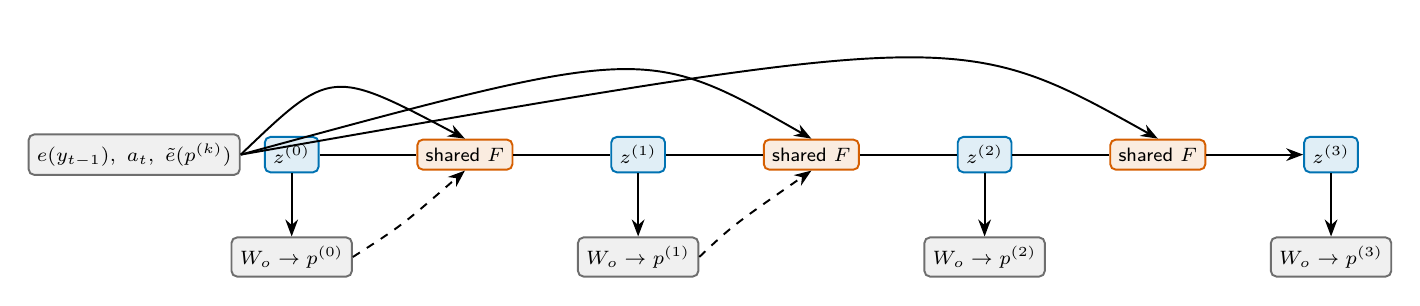
\begin{tikzpicture}[font=\sffamily\scriptsize, >=Stealth, line width=0.7pt,
  b/.style={draw, rounded corners=2pt, align=center, inner sep=3pt},
  u/.style={b, draw=oiBlue, fill=oiBlue!12},
  g/.style={b, draw=oiGray, fill=oiGray!10},
  o/.style={b, draw=oiOrange, fill=oiOrange!12}]
\node[g] (inp) at (0,0) {$e(y_{t-1}),\ a_t,\ \tilde e(p^{(k)})$};
\node[u] (z0) at (2.0,0) {$z^{(0)}$};
\node[o] (r0) at (4.2,0) {shared $F$};
\node[u] (z1) at (6.4,0) {$z^{(1)}$};
\node[o] (r1) at (8.6,0) {shared $F$};
\node[u] (z2) at (10.8,0) {$z^{(2)}$};
\node[o] (r2) at (13.0,0) {shared $F$};
\node[u] (z3) at (15.2,0) {$z^{(3)}$};
\node[g] (o0) at (2.0,-1.3) {$W_o \to p^{(0)}$};
\node[g] (o1) at (6.4,-1.3) {$W_o \to p^{(1)}$};
\node[g] (o2) at (10.8,-1.3) {$W_o \to p^{(2)}$};
\node[g] (o3) at (15.2,-1.3) {$W_o \to p^{(3)}$};
\draw[->] (z0) -- (r0) -- (z1) -- (r1) -- (z2) -- (r2) -- (z3);
\draw[->] (inp.east) .. controls (2.5,1.1) .. (r0.north);
\draw[->] (inp.east) .. controls (6.5,1.4) .. (r1.north);
\draw[->] (inp.east) .. controls (10.5,1.6) .. (r2.north);
\draw[->] (z0) -- (o0); \draw[->] (z1) -- (o1); \draw[->] (z2) -- (o2); \draw[->] (z3) -- (o3);
\draw[->,dashed] (o0.east) .. controls (3.4,-0.9) .. (r0.south);
\draw[->,dashed] (o1.east) .. controls (7.6,-0.9) .. (r1.south);
\end{tikzpicture}%
}
\caption{某输出位置上的递归精化。基步产生 $z^{(0)}$；共享算子 $F$ 用上一词元嵌入、基步注意力上下文与当前预测的软嵌入 $p^{(k)}E$ 把 $z^{(k)}$ 映射为 $z^{(k+1)}$。共享输出头在每个深度给出分布，参数量不随深度增加。}
\label{fig:refine}
\end{figure}

这四类转移是词元级的，因此可以逐个词元决定是否再花一次计算。因果停算在展开的两个点上做决定：基步之后，以及第一次精化之后。每处都把当前预测的 top-1 概率与固定阈值比较。概率超过阈值时该词元停下；两个阈值在所有模型与种子上固定为 $0.85$ 与 $0.90$。每次决定只使用它门控的精化之前就已算出的信号，因此停下的词元不会读取它选择跳过的计算。通过两道门控的词元继续走到 $e_3$。

预测的退出深度与实际执行的调用是两回事。调用数需要单独测量：执行器在每次基步调用前收集活跃行，在每次精化调用前收集继续解码的行，再把输出写回批次，使已完成与已停下的行不进入任何调用。$N_{\mathrm{cell}}$ 定义为执行器实际发出的调用：每个活跃行一次基步调用，加上该行执行的每次精化各一次调用。解码器与精化单元上的前向钩子记录每次调用的输入行数。当钩子计数与 $N_{\mathrm{cell}}$ 一致时，调用计数的下降就反映了执行器确实没有执行的计算。

\begin{figure}[H]
\centering
\resizebox{\columnwidth}{!}{%
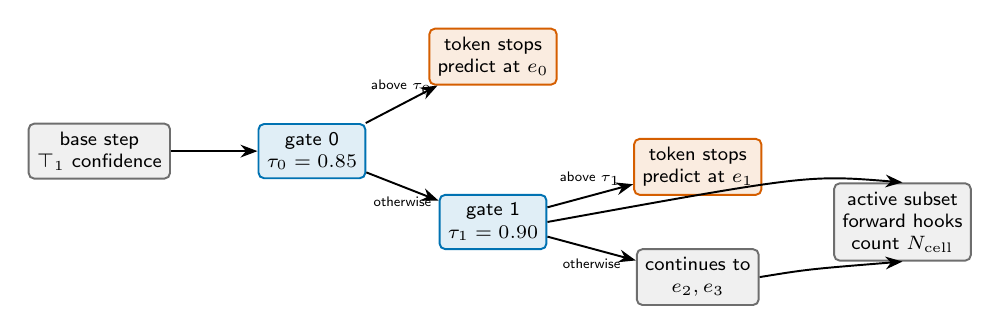
\begin{tikzpicture}[font=\sffamily\scriptsize, >=Stealth, line width=0.7pt,
  b/.style={draw, rounded corners=2pt, align=center, inner sep=3pt},
  u/.style={b, draw=oiBlue, fill=oiBlue!12},
  g/.style={b, draw=oiGray, fill=oiGray!10},
  r/.style={b, draw=oiOrange, fill=oiOrange!12}]
\node[g] (base) at (0,0) {base step\\$\top_1$ confidence};
\node[u] (g0) at (2.7,0) {gate 0\\$\tau_0=0.85$};
\node[r] (s0) at (5.0,1.2) {token stops\\predict at $e_0$};
\node[u] (g1) at (5.0,-0.9) {gate 1\\$\tau_1=0.90$};
\node[r] (s1) at (7.6,-0.2) {token stops\\predict at $e_1$};
\node[g] (deep) at (7.6,-1.6) {continues to\\$e_2,e_3$};
\node[g] (audit) at (10.2,-0.9) {active subset\\
forward hooks\\count $N_{\mathrm{cell}}$};
\draw[->] (base) -- (g0);
\draw[->] (g0) -- node[above,font=\sffamily\tiny] {above $\tau_0$} (s0);
\draw[->] (g0) -- node[below,font=\sffamily\tiny] {otherwise} (g1);
\draw[->] (g1) -- node[above,font=\sffamily\tiny] {above $\tau_1$} (s1);
\draw[->] (g1) -- node[below,font=\sffamily\tiny] {otherwise} (deep);
\draw[->] (g1.east) .. controls (9.0,-0.3) .. (audit.north);
\draw[->] (deep.east) .. controls (9.0,-1.5) .. (audit.south);
\end{tikzpicture}%
}
\caption{因果词元级停算。每道门控只读取其所控制的精化之前已算出的信号，停下的词元不会使用被跳过的计算。预测的退出深度与实际执行的调用不是同一个量：active-subset 执行器只对继续解码的行运行单元，前向钩子核对拦截到的调用数与 $N_{\mathrm{cell}}$ 一致。}
\label{fig:halt}
\end{figure}

停算决定何时停止，却不说明一次精化对状态做了什么。每个生成位置与深度都记录潜向量，连同预测分布与预测词元，得到每个词元的一条轨迹 $z^{(0)},\dots,z^{(3)}$。记录在固定的组均衡源样本上以自由运行的贪心解码进行，并逐个模型施加；teacher forcing 只用于训练期诊断，不用于这些轨迹。

从每条轨迹计算六个摘要：归一化状态范数 $\lVert z_k\rVert/\sqrt d$、更新范数、相对更新、相邻更新的余弦、相对 $z^{(0)}$ 的总位移，以及预测词元跨深度变化的比率。词元级数值先在样本内平均，再按组做簇自助得到 95\% 区间。LSTM 的隐状态与细胞状态分开，Mamba 的解码器潜状态与其内部 SSM 状态分开；Mamba 是单种子描述性探针，不进入主表。

精化规则本身未必是最好的更新。在固定深度下，把每一步改写为 $z^{(k+1)}=z^{(k)}+\alpha^{(k)}\Delta z^{(k)}$，其中 $\alpha^{(k)}=\sigma(w_0+w_1\tilde H+w_2\tilde D+w_3\tilde A+w_4\,k/K)$：一个截距项加上四个因果可得特征，预测熵 $H$、更新幅度 $D$、更新方向 $A$ 与深度 $k/K$。搜索只改变这五个系数；模型权重与精化步数保持不变，因此准确率变化是在恒定计算下的潜状态动力学效应。

\begin{figure}[H]
\centering
\resizebox{\columnwidth}{!}{%
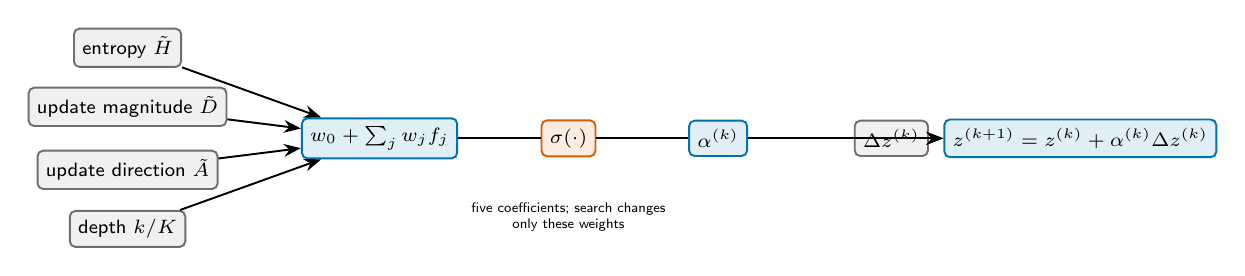
\begin{tikzpicture}[font=\sffamily\scriptsize, >=Stealth, line width=0.7pt,
  b/.style={draw, rounded corners=2pt, align=center, inner sep=3pt},
  g/.style={b, draw=oiGray, fill=oiGray!10},
  u/.style={b, draw=oiBlue, fill=oiBlue!12},
  o/.style={b, draw=oiOrange, fill=oiOrange!12}]
\node[g] (H) at (0,1.15) {entropy $\tilde H$};
\node[g] (D) at (0,0.4) {update magnitude $\tilde D$};
\node[g] (A) at (0,-0.4) {update direction $\tilde A$};
\node[g] (k) at (0,-1.15) {depth $k/K$};
\node[u] (lin) at (3.2,0) {$w_0+\sum_j w_j f_j$};
\node[o] (sig) at (5.6,0) {$\sigma(\cdot)$};
\node[u] (a) at (7.5,0) {$\alpha^{(k)}$};
\node[g] (dz) at (9.7,0) {$\Delta z^{(k)}$};
\node[u] (eq) at (12.1,0) {$z^{(k+1)}=z^{(k)}+\alpha^{(k)}\Delta z^{(k)}$};
\draw[->] (H) -- (lin); \draw[->] (D) -- (lin); \draw[->] (A) -- (lin); \draw[->] (k) -- (lin);
\draw[->] (lin) -- (sig) -- (a) -- (eq); \draw[->] (dz) -- (eq);
\node[font=\sffamily\tiny,align=center] at (5.6,-1.0) {five coefficients; search changes\\only these weights};
\end{tikzpicture}%
}
\caption{进化式潜状态步长控制。四个因果可得特征与一个截距项构成五维策略；sigmoid 将其映射为 $\alpha^{(k)}$，用于缩放固定深度下的精化位移。模型权重与精化步数不变，因此准确率变化只来自更新规则。}
\label{fig:alpha}
\end{figure}

五种算法在同一预算 336 次评估下搜索同一策略：随机搜索、遗传算法、变异引导变体、差分进化与 sep-CMA-ES。对每个模型种子，取内层折上的最优策略，冻结其权重与特征归一化统计量，并在 640 样本的外层折上确认一次。再把该冻结策略原样用于 Vanilla RNN、LSTM 与 Transformer，不再搜索，并报告哪些种子非劣、哪些不是。

图~\ref{fig:method_overview} 把三个组件放在同一条时间线上。面板~(a) 区分了预测层面的问题与执行层面的问题：门控决定额外的精化是否值得运行，而钩子审计验证被跳过的调用是否真的从执行路径中消失。面板~(b) 固定深度，使更新规则的效果不与额外步骤的效果混淆，并给出该规则被检验的位置：一次留出折确认，以及在未见架构上不做重新搜索的迁移。本节余下部分按图中顺序逐一定义各组件。

面板~(a) 从左到右阅读。冻结递归 GRU 的基步产生 $e_0$ 与 top-1 置信度；门控 0 把它与 $\tau_0=0.85$ 比较，超过阈值的词元在精化 1 运行之前停下。继续的词元到达 $e_1$，门控 1 用 $\tau_1=0.90$ 重复判断，只有剩余的行进入后续两次精化直至 $e_3$。被审计的计数器因此记录每个活跃行一次基步调用，再加上该行实际执行的每次精化调用；这正是第~\ref{sec:results} 章各系统之间比较的量。面板~(b) 按同样方向阅读：当前状态与前缀给出熵 $\tilde H$、更新幅度 $\tilde D$、更新方向 $\tilde A$ 与深度 $k/K$；冻结单元提供未缩放的位移 $\Delta z_i^{(k)}$；策略把它们映射为 $\alpha_i^{(k)}$，由调制后的精化在恒定 $N_{\mathrm{cell}}$ 下施加。五种算法在 336 次评估预算下搜索五个系数，选出的策略被冻结后才进行面板右侧所示的外层确认与跨架构迁移。

\begin{figure*}[t]
\centering
\resizebox{\textwidth}{!}{%
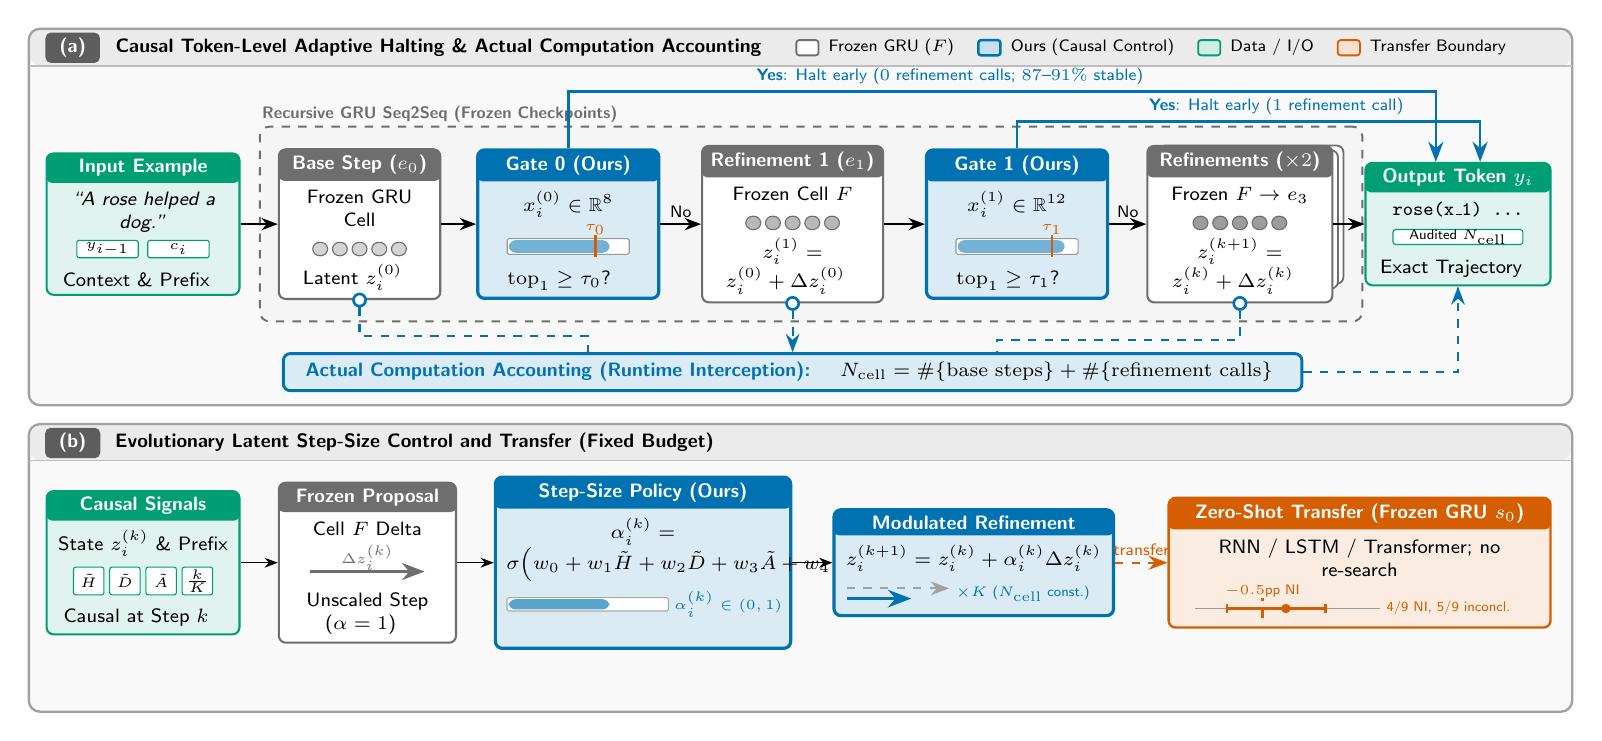
\begin{tikzpicture}[
    font=\sffamily\fontsize{6.8pt}{8.2pt}\selectfont,
    >=Stealth,
    line width=0.65pt,
    % Card Styles
    cardBlue/.style={
        draw=oiBlue, fill=oiBlue!14,
        line width=1.15pt, rounded corners=2.5pt, inner sep=0pt
    },
    cardGray/.style={
        draw=oiGray, fill=white,
        line width=0.75pt, rounded corners=2.5pt, inner sep=0pt
    },
    cardGreen/.style={
        draw=oiGreen, fill=oiGreen!12,
        line width=0.75pt, rounded corners=2.5pt, inner sep=0pt
    },
    cardOrange/.style={
        draw=oiOrange, fill=oiOrange!12,
        line width=0.85pt, rounded corners=2.5pt, inner sep=0pt
    },
    hdr/.style={
        font=\sffamily\fontsize{6.6pt}{7.8pt}\selectfont\bfseries,
        text=white, align=center, inner xsep=2pt, inner ysep=2.2pt,
        rounded corners=1.8pt
    },
    probe/.style={
        circle, draw=oiBlue, fill=white, line width=0.95pt,
        minimum size=4.4pt, inner sep=0pt
    },
    panelBadge/.style={
        font=\sffamily\fontsize{7pt}{8pt}\selectfont\bfseries,
        text=white, fill=oiGray!85!black, rounded corners=2pt, inner xsep=5pt, inner ysep=2pt
    },
    panelTitle/.style={
        font=\sffamily\fontsize{7.5pt}{9pt}\selectfont\bfseries,
        text=black, inner sep=0pt
    },
    tag/.style={font=\sffamily\fontsize{5.8pt}{6.8pt}\selectfont, inner sep=1pt}
]

% Two-tone Header Card Macro
\newcommand{\richcard}[7]{
    \node[#4] (#1) at (#2) {
        \begin{minipage}{#3}
            \centering
            \tikz{\node[hdr, fill=#5, minimum width=#3, text width=\dimexpr#3-4pt\relax] {#6};}\\[-0.5pt]
            \begin{minipage}{\dimexpr#3-8pt\relax}
                \vspace{3pt}\centering #7 \vspace{3pt}
            \end{minipage}
        \end{minipage}
    };
}

\def\xLeft{-0.25}
\def\xRight{19.35}

% ==============================================================================
% PANEL (a) CONTENT
% ==============================================================================
\node[panelBadge, anchor=west] (badgeA) at (-0.05, 5.02) {(a)};
\node[panelTitle, right=5pt of badgeA] (titleA) {Causal Token-Level Adaptive Halting \& Actual Computation Accounting};

% Legend placed directly after titleA with normal spacing
\node[draw=oiGray, fill=white, minimum width=8pt, minimum height=5.5pt, inner sep=0pt, rounded corners=1pt, right=12pt of titleA] (l1) {};
\node[tag, right=2pt of l1] (l1t) {Frozen GRU ($F$)};
\node[draw=oiBlue, fill=oiBlue!22, line width=0.9pt, minimum width=8pt, minimum height=5.5pt, inner sep=0pt, rounded corners=1pt, right=7pt of l1t] (l2) {};
\node[tag, right=2pt of l2] (l2t) {Ours (Causal Control)};
\node[draw=oiGreen, fill=oiGreen!18, minimum width=8pt, minimum height=5.5pt, inner sep=0pt, rounded corners=1pt, right=7pt of l2t] (l3) {};
\node[tag, right=2pt of l3] (l3t) {Data / I/O};
\node[draw=oiOrange, fill=oiOrange!18, minimum width=8pt, minimum height=5.5pt, inner sep=0pt, rounded corners=1pt, right=7pt of l3t] (l4) {};
\node[tag, right=2pt of l4] (l4t) {Transfer Boundary};

\def\yA{2.78}

% 1. Input Card (Green)
\richcard{inA}{1.20, \yA}{2.45cm}{cardGreen}{oiGreen}{Input Example}{
    \textit{``A rose helped a dog.''}\\[2.5pt]
    \tikz{
        \foreach \x/\lbl in {0/$y_{i-1}$, 0.90/$c_i$} {
            \draw[draw=oiGreen, fill=white, rounded corners=0.8pt] (\x,0) rectangle ++(0.78, 0.22);
            \node[font=\sffamily\fontsize{5.3pt}{5.3pt}\selectfont] at (\x+0.39, 0.11) {\lbl};
        }
    }\\[2pt]
    Context \& Prefix
}

% 2. Base Step e_0 (Gray)
\richcard{baseA}{3.95, \yA}{2.05cm}{cardGray}{oiGray}{Base Step ($e_0$)}{
    Frozen GRU Cell\\[2.5pt]
    \tikz{
        \foreach \k in {0,1,2,3,4} {
            \draw[draw=oiGray, fill=oiGray!30] (\k*0.25,0) rectangle ++(0.19, 0.17);
        }
    }\\[2pt]
    Latent $z_i^{(0)}$
}

% 3. Gate 0 (Blue - Ours)
\richcard{gate0}{6.60, \yA}{2.30cm}{cardBlue}{oiBlue}{Gate 0 (Ours)}{
    $x_i^{(0)} \in \mathbb{R}^8$\\[1.5pt]
    \tikz{
        \node[font=\sffamily\fontsize{5.2pt}{5.2pt}\selectfont, text=oiOrange, anchor=south] at (1.12, 0.24) {$\tau_0$};
        \draw[draw=oiGray!70, fill=white, rounded corners=0.6pt] (0,0) rectangle (1.55, 0.20);
        \fill[oiBlue!55] (0.02,0.02) rectangle (1.30, 0.18);
        \draw[draw=oiOrange, line width=0.95pt] (1.12, -0.03) -- (1.12, 0.24);
    }\\[1.5pt]
    $\mathrm{top}_1 \ge \tau_0$?
}

% 4. Refinement 1 e_1 (Gray)
\richcard{ref1}{9.45, \yA}{2.30cm}{cardGray}{oiGray}{Refinement 1 ($e_1$)}{
    Frozen Cell $F$\\[2.5pt]
    \tikz{
        \foreach \k in {0,1,2,3,4} {
            \draw[draw=oiGray, fill=oiGray!48] (\k*0.25,0) rectangle ++(0.19, 0.17);
        }
    }\\[2pt]
    $z_i^{(1)} = z_i^{(0)} + \Delta z_i^{(0)}$
}

% 5. Gate 1 (Blue - Ours)
\richcard{gate1}{12.30, \yA}{2.30cm}{cardBlue}{oiBlue}{Gate 1 (Ours)}{
    $x_i^{(1)} \in \mathbb{R}^{12}$\\[1.5pt]
    \tikz{
        \node[font=\sffamily\fontsize{5.2pt}{5.2pt}\selectfont, text=oiOrange, anchor=south] at (1.22, 0.24) {$\tau_1$};
        \draw[draw=oiGray!70, fill=white, rounded corners=0.6pt] (0,0) rectangle (1.55, 0.20);
        \fill[oiBlue!55] (0.02,0.02) rectangle (1.38, 0.18);
        \draw[draw=oiOrange, line width=0.95pt] (1.22, -0.03) -- (1.22, 0.24);
    }\\[1.5pt]
    $\mathrm{top}_1 \ge \tau_1$?
}

% 6. Remaining Refinements x2 -> e_3 (Stacked Gray Cards)
\node[draw=oiGray, fill=white, rounded corners=2.5pt, minimum width=2.35cm, minimum height=50pt] (refK_s2) at (15.27, \yA+0.12) {};
\node[draw=oiGray, fill=white, rounded corners=2.5pt, minimum width=2.35cm, minimum height=50pt] (refK_s1) at (15.20, \yA+0.06) {};
\richcard{refK}{15.13, \yA}{2.35cm}{cardGray}{oiGray}{Refinements ($\times 2$)}{
    Frozen $F \rightarrow e_3$\\[2.5pt]
    \tikz{
        \foreach \k in {0,1,2,3,4} {
            \draw[draw=oiGray, fill=oiGray!68] (\k*0.25,0) rectangle ++(0.19, 0.17);
        }
    }\\[2pt]
    $z_i^{(k+1)} = z_i^{(k)} + \Delta z_i^{(k)}$
}

% 7. Output Card (Green)
\richcard{outA}{17.90, \yA}{2.35cm}{cardGreen}{oiGreen}{Output Token $y_i$}{
    \texttt{rose(x\_1) ...}\\[2.5pt]
    \tikz{
        \draw[draw=oiGreen, fill=white, rounded corners=1pt] (0,0) rectangle (1.65, 0.19);
        \node[font=\sffamily\fontsize{5.3pt}{5.3pt}\selectfont, text=black] at (0.825, 0.095) {Audited $N_{\mathrm{cell}}$};
    }\\[2pt]
    Exact Trajectory
}

% Main Pipeline Arrows
\draw[->] (inA.east) -- (baseA.west);
\draw[->] (baseA.east) -- (gate0.west);
\draw[->] (gate0.east) -- node[tag, above=1pt] {No} (ref1.west);
\draw[->] (ref1.east) -- (gate1.west);
\draw[->] (gate1.east) -- node[tag, above=1pt] {No} (refK.west);
\draw[->] (refK.east) -- (outA.west);

% Top Early-Exit Rails (Blue)
\draw[->, draw=oiBlue, line width=0.95pt]
    (gate0.north) -- ++(0, 0.72) -| node[tag, pos=0.22, above=1pt, text=oiBlue] {\textbf{Yes}: Halt early ($0$ refinement calls; $87\text{--}91\%$ stable)} ([xshift=-8pt]outA.north);

\draw[->, draw=oiBlue, line width=0.95pt]
    (gate1.north) -- ++(0, 0.34) -| node[tag, pos=0.28, above=1pt, text=oiBlue] {\textbf{Yes}: Halt early ($1$ refinement call)} ([xshift=8pt]outA.north);

% Runtime Interception Audit Bus (Bottom)
\node[draw=oiBlue, fill=oiBlue!14, line width=1.05pt, rounded corners=2.5pt, inner xsep=8pt, inner ysep=3.2pt, align=center] (counter) at (9.45, 0.90) {
    \textbf{\textcolor{oiBlue}{Actual Computation Accounting (Runtime Interception):}} \quad
    $N_{\mathrm{cell}} = \#\{\mathrm{base\ steps}\} + \#\{\mathrm{refinement\ calls}\}$
};

% Interception Probes on Frozen Modules
\node[probe] (pr1) at (baseA.south) {};
\node[probe] (pr2) at (ref1.south) {};
\node[probe] (pr3) at (refK.south) {};

\draw[dashed, draw=oiBlue, line width=0.8pt] (pr1) -- ++(0, -0.46) -| ([xshift=-2.6cm]counter.north);
\draw[->, dashed, draw=oiBlue, line width=0.8pt] (pr2) -- (pr2 |- counter.north);
\draw[dashed, draw=oiBlue, line width=0.8pt] (pr3) -- ++(0, -0.46) -| ([xshift=2.6cm]counter.north);
\draw[->, dashed, draw=oiBlue, line width=0.8pt] (counter.east) -| (outA.south);

% Background layers for Panel (a)
\begin{pgfonlayer}{background}
    % Outer Panel (a) Frame
    \draw[draw=oiGray!65, fill=oiGray!4, line width=0.85pt, rounded corners=4pt]
        (\xLeft, 0.48) rectangle (\xRight, 5.26);
    \fill[oiGray!14, rounded corners=3.5pt] (\xLeft+0.02, 4.79) rectangle (\xRight-0.02, 5.24);
    \draw[draw=oiGray!45, line width=0.5pt] (\xLeft, 4.79) -- (\xRight, 4.79);

    % Inner Zone Box for Recursive GRU Seq2Seq
    \node[draw=oiGray, fill=oiGray!7, dashed, line width=0.7pt, rounded corners=3.5pt, inner sep=6.5pt,
          fit=(baseA)(ref1)(refK)(refK_s2),
          label={[tag, text=oiGray, anchor=south west]north west:\textbf{Recursive GRU Seq2Seq (Frozen Checkpoints)}}] {};
\end{pgfonlayer}


% ==============================================================================
% PANEL (b) CONTENT
% ==============================================================================
\node[panelBadge, anchor=west] (badgeB) at (-0.05, 0.00) {(b)};
\node[panelTitle, right=5pt of badgeB] (titleB) {Evolutionary Latent Step-Size Control and Transfer (Fixed Budget)};

\def\yB{-1.52}

% 1. Causal Signals (Green)
\richcard{inB}{1.20, \yB}{2.45cm}{cardGreen}{oiGreen}{Causal Signals}{
    State $z_i^{(k)}$ \& Prefix\\[2.5pt]
    \tikz{
        \foreach \lbl/\x in {$\tilde{H}$/0, $\tilde{D}$/0.46, $\tilde{A}$/0.92, $\frac{k}{K}$/1.38} {
            \node[draw=oiGreen, fill=white, rounded corners=0.8pt, minimum width=11pt, minimum height=10pt, inner sep=0.5pt, font=\sffamily\fontsize{5.4pt}{5.4pt}\selectfont] at (\x+0.2, 0.1) {\lbl};
        }
    }\\[1.5pt]
    Causal at Step $k$
}

% 2. Frozen Cell Update Proposal (Gray)
\richcard{propB}{4.05, \yB}{2.25cm}{cardGray}{oiGray}{Frozen Proposal}{
    Cell $F$ Delta\\[2.5pt]
    \tikz{
        \draw[->, draw=oiGray, line width=1.15pt] (0,0.08) -- (1.45,0.08);
        \node[font=\sffamily\fontsize{5.5pt}{5.5pt}\selectfont, text=oiGray, above] at (0.725, 0.08) {$\Delta z_i^{(k)}$};
    }\\[1.5pt]
    Unscaled Step ($\alpha=1$)
}

% 3. Step-Size Policy (Blue - Ours)
\richcard{stepB}{7.55, \yB}{3.75cm}{cardBlue}{oiBlue}{Step-Size Policy (Ours)}{
    $\alpha_i^{(k)} = \sigma\!\left(w_0 + w_1\tilde{H} + w_2\tilde{D} + w_3\tilde{A} + w_4\frac{k}{K}\right)$\\[2.5pt]
    \tikz{
        \draw[draw=oiGray!60, fill=white, rounded corners=0.6pt] (0,0) rectangle (2.05, 0.17);
        \fill[oiBlue!65] (0.02,0.02) rectangle (1.30, 0.15);
        \node[font=\sffamily\fontsize{5.3pt}{5.3pt}\selectfont, text=oiBlue, anchor=west] at (2.12, 0.085) {$\alpha_i^{(k)} \in (0,1)$};
    }
}

% 4. Modulated Refinement (Blue - Ours)
\richcard{modB}{11.75, \yB}{3.55cm}{cardBlue}{oiBlue}{Modulated Refinement}{
    $z_i^{(k+1)} = z_i^{(k)} + \alpha_i^{(k)}\Delta z_i^{(k)}$\\[2.5pt]
    \tikz{
        \draw[->, draw=oiGray!65, dashed, line width=0.8pt] (0,0.16) -- (1.30,0.16);
        \draw[->, draw=oiBlue, line width=1.2pt] (0,0.03) -- (0.82,0.03);
        \node[font=\sffamily\fontsize{5.3pt}{5.3pt}\selectfont, text=oiBlue, anchor=west] at (1.38, 0.095) {$\times K$ ($N_{\mathrm{cell}}$ const.)};
    }
}

% 5. Transfer boundary (Orange)
\richcard{jointB}{16.65, \yB}{4.85cm}{cardOrange}{oiOrange}{Zero-Shot Transfer (Frozen GRU $s_0$)}{
    RNN / LSTM / Transformer; no re-search\\[2pt]
    \tikz{
        \node[font=\sffamily\fontsize{5.1pt}{5.1pt}\selectfont, text=oiOrange, anchor=south] at (0.85, 0.24) {$-0.5\text{pp}$ NI};
        \draw[draw=oiGray!70] (0,0.10) -- (2.35,0.10);
        \draw[draw=oiOrange, dashed, line width=0.9pt] (0.85, -0.02) -- (0.85, 0.23);
        \draw[draw=oiOrange, line width=1.15pt] (0.40, 0.10) -- (1.65, 0.10);
        \draw[draw=oiOrange, line width=0.9pt] (0.40, 0.04) -- (0.40, 0.16);
        \draw[draw=oiOrange, line width=0.9pt] (1.65, 0.04) -- (1.65, 0.16);
        \fill[oiOrange] (1.15, 0.10) circle (1.7pt);
        \node[font=\sffamily\fontsize{5.3pt}{5.3pt}\selectfont, text=oiOrange, anchor=west] at (2.42, 0.10) {4/9 NI, 5/9 inconcl.};
    }
}

% Panel (b) Flow Arrows
\draw[->] (inB.east) -- (propB.west);
\draw[->] (propB.east) -- (stepB.west);
\draw[->] (stepB.east) -- (modB.west);
\draw[->, dashed, draw=oiOrange, line width=0.85pt] (modB.east) -- node[tag, above=1pt, text=oiOrange] {transfer} (jointB.west);

% Background layers for Panel (b)
\begin{pgfonlayer}{background}
    % Inner Zone Box for Constant-Compute Control
    \node[draw=oiBlue, fill=oiBlue!6, dashed, line width=0.85pt, rounded corners=3.5pt, inner sep=6pt,
          fit=(stepB)(modB)] (zoneB) {};
    \node[tag, text=oiBlue, anchor=north] (zoneBLabel) at ($(zoneB.south)+(0,-1.5pt)$) {\textbf{Fixed-Depth Latent Dynamics Control (Ours)}};

    % Outer Panel (b) Frame (Dynamically encloses zoneBLabel with generous bottom margin)
    \path let \p1 = (zoneBLabel.south) in
        node[draw=oiGray!65, fill=oiGray!4, line width=0.85pt, rounded corners=4pt, inner sep=0pt,
             fit={(\xLeft, \y1-6pt) (\xRight, 0.24)}] (panelBBox) {};
    \fill[oiGray!14, rounded corners=3.5pt] (\xLeft+0.02, -0.22) rectangle (\xRight-0.02, 0.22);
    \draw[draw=oiGray!45, line width=0.5pt] (\xLeft, -0.22) -- (\xRight, -0.22);
\end{pgfonlayer}

\end{tikzpicture}%
}
\caption{\textbf{TRACER 总览：追踪、停算与控制递归计算。} \textbf{(a)} 在词元 $i$ 上，冻结的递归 GRU 产生 $e_0,e_1,e_3$ 三个深度（灰色）。两道因果置信门控（蓝色）只读取其所控制的精化之前就已可得的前缀信号 $x_i^{(0)},x_i^{(1)}$，因此停下的词元不会进入被跳过的调用。运行时拦截（绿色）统计真实的基步与精化调用，得到 $N_{\mathrm{cell}}$，而不是推断出的退出深度。\textbf{(b)} 在固定深度下，五参数策略把预测熵、更新幅度、更新方向与深度映射为步长 $\alpha_i^{(k)}\in(0,1)$，在不改变 $N_{\mathrm{cell}}$ 的前提下缩放精化位移。该策略在冻结后只做一次外层确认，并在不做重新搜索的情况下迁移；迁移只覆盖部分目标种子（九个中四个非劣），这标出了所学规则的边界。}
\label{fig:method_overview}
\end{figure*}

\section{实验}
\label{sec:exp}

我们在 COGS 上评估 TRACER，这是一个把自然语言映射为逻辑形式的语义解析基准。实验围绕三个问题展开：额外步骤究竟执行了什么，它们改变了潜状态的什么，以及步长策略能否迁移。三条主线共享冻结检查点与统一的执行调用定义，但数据划分各不相同；非劣效判据用于停算与消融中的策略确认。

\subsection{数据集}
COGS 通过把自然语言映射为逻辑形式来测试组合泛化 \citep{kim2020cogs}。更宽泛的系统泛化困难 \citep{keysers2020measuring,furrer2020compositional} 推动了结构化解析器 \citep{herzig2021span,shaw2021compositional} 与解耦模型 \citep{zheng2022disentangled}，但单纯扩大规模并不能消除它 \citep{qiu2022evaluating,li2023slog}，COGS 仍是标准基准 \citep{weissenhorn2022compositional}。COGS 包含 24,155 个训练样本、3,000 个开发样本、3,000 个测试样本与 21,000 个泛化样本；官方测试与泛化划分保持封存，从未读取。跨架构评估与潜状态分析共享一个固定的、组均衡的 256 个主训练样本，所有主模型与种子都使用它。优化器搜索在一个搜索前固定的内层子集上进行，选出的每个策略只在一个约 640 个训练样本的外层折上确认一次。另做一次最终检查：仅将已冻结的阈值策略用于官方 3,000 样本开发集，评估一次后即标记为已使用，不再触碰。

\subsection{实验环境}
所有实验在同一台本地 CPU 工作站上完成，所有计时均固定使用两个线程。GRU、Vanilla RNN、LSTM 与 Transformer 各训练三个种子，另有一个单种子 Mamba-1-Tiny 作为边界探针（表~\ref{tab:models}）。训练使用 Adam、学习率 $10^{-3}$、批大小 32、15 个 epoch，GRU 系列模型使用 64 维嵌入与 128 维隐状态；递归 Transformer 则采用 128 维宽度。精化最多三步，在多深度监督下按 $(0.1,0.2,0.3,0.4)$ 加权覆盖 $e_0$--$e_3$，模型种子为 0、1、2。五种算法各用三个优化器种子搜索，每次运行 336 次候选评估。非劣效成立的条件是：对 $\Delta$EM 的 95\% 组簇自助区间下界达到 $-0.5$pp 或以上；仅凭点估计不作判定。

\begin{table}[H]
\centering
\small
\begin{tabular}{llc}
\toprule
模型 & 核心结构 & 参数量 \\
\midrule
GRU & GRUCell + Bahdanau attn & 560K \\
Vanilla RNN & RNNCell + dot attn & 343K \\
LSTM & LSTMCell + dot attn & 689K \\
Transformer & 递归，宽度 128 & 799K \\
Mamba & Mamba-1 S6，64 & 149K \\
\bottomrule
\end{tabular}
\caption{架构配置。Mamba 为单种子边界探针。}
\label{tab:models}
\end{table}

\subsection{实验设计}
TRACER 的三条主线层层递进。深度研究刻画每个递归深度的贡献，为因果停算提供依据；停算与消融据此确认哪些步骤该运行、哪些被跳过。潜状态研究把问题推进到状态本身，追问额外步骤改变了什么。步长搜索最后固定深度，检验一个更新策略能在留出数据与未见架构上走多远。三条主线共享冻结检查点与统一的执行调用定义；两条诊断主线读取共同的 256 样本 manifest，搜索使用自己的内层和外层折。

深度研究为四个主架构各训练三个种子，在同一批 256 个组均衡样本上解码 $e_0$ 至 $e_3$。对每一对相邻深度，统计结果落入修复、损害、保持未变、仍未解决中的哪一类。把准确率对深度作图，可以看出增益在何处饱和，以及模型已稳定后精化仍在何处改变预测。

停算研究在这条展开上放置两道门控，分别在基步之后与第一次精化之后，固定阈值为 $0.85$ 与 $0.90$。我们把停算解码与强制 $e_3$ 以及每个种子各自的最佳固定深度比较，报告 EM、配对自助区间与 $N_{\mathrm{cell}}$。带前向钩子的 active-subset 执行器检查被跳过的精化是否真的没有触发调用。我们还对批大小 1、4、8、32 计时，考察调用节省在多大程度上转化为真实墙钟时间的下降；Transformer 使用自己的逐样本解码器，单独报告。

消融分开回答两个问题。在共享的 256 样本协议下，我们把固定阈值与强制停（$e_0$）、强制继续（$e_3$）对照，并用钩子计数确认被省略的精化确实没有执行；这排除了记账造成的假象。在另一套单架构 GRU 设置（fold-4，每种子 645 样本）上，对阈值对的描述性扫描，以及 top-1、margin 与熵读数的比较，表明固定阈值落在一段平坦的非劣区间内；两项扫描都不重新选择策略。

停算改变的是哪些步骤运行，而不是一步对状态做了什么。潜状态研究使用 256 样本 manifest，记录四个主架构各三个种子的 $e_0$--$e_3$ 轨迹。每个词元贡献一个状态向量、由预测分布导出的量以及它的预测。我们在每个深度计算六个摘要统计量，先在样本内平均，再按组重采样得到置信区间。LSTM 的隐状态与细胞状态保持分开。

我们把四个架构的轨迹画在同一组面板里，检查第一次精化的模式是否跨种子一致。两类状态分开处理：有界门控态（GRU、Vanilla RNN、LSTM 隐状态）与持续增长的累积态（LSTM 细胞状态、Transformer）。这些是描述性比较，不是受控的单元消融，因为注意力类型与参数量也同时变化。单种子 Mamba 探针提供 64 样本的描述，记录其解码器潜状态与内部 SSM 状态，不进入四架构统计。

搜索固定递归深度与模型权重。参数化策略在每次精化时缩放更新步长，五种算法（随机搜索、遗传算法、变异引导变体、差分进化、sep-CMA-ES）各用每个模型种子的三个优化器种子搜索，每次运行 336 次评估。基线是原始更新 $\alpha\equiv1$，因此任何增益都在恒定深度下隔离出步长效应。

我们对策略输入做三组消融：深度索引、预测熵、潜状态动力学特征（更新幅度与方向）。同时记录各深度选出的 $\alpha$ 与预测发生改变的词元，以判断增益来自深度调度还是内容依赖的更新。消融并没有唯一地支持其中一种解释。

内层最优策略被冻结后，在 640 样本的外层折上确认一次。这一条 GRU 策略及其特征归一化统计量随后原样用于 Vanilla RNN、LSTM 与 Transformer 的全部三个种子，不再搜索。每个目标种子按非劣效界分类；既不满足非劣效也未显著变差的种子记为不确定。

三条主线合成一套叙述。潜状态曲线解释为什么在深度一已经饱和处停算是安全的，调用计数说明节省由什么构成，步长搜索给出冻结更新策略在恒定深度下的增益范围以及迁移何时开始失效。我们把负面案例与正面案例放在一起报告。

\section{结果与实验分析}
\label{sec:results}

三条问题组织本节：被计数的额外步骤是否真的执行、潜状态内部发生了什么、调整后的更新规则能否迁移。以下每个结论都有从公开结果文件计算得到的表或图支撑，负面与不确定结果和正面结果在同一段落中报告。

\textbf{递归计算与因果停算。} \begin{figure}[H]
\centering
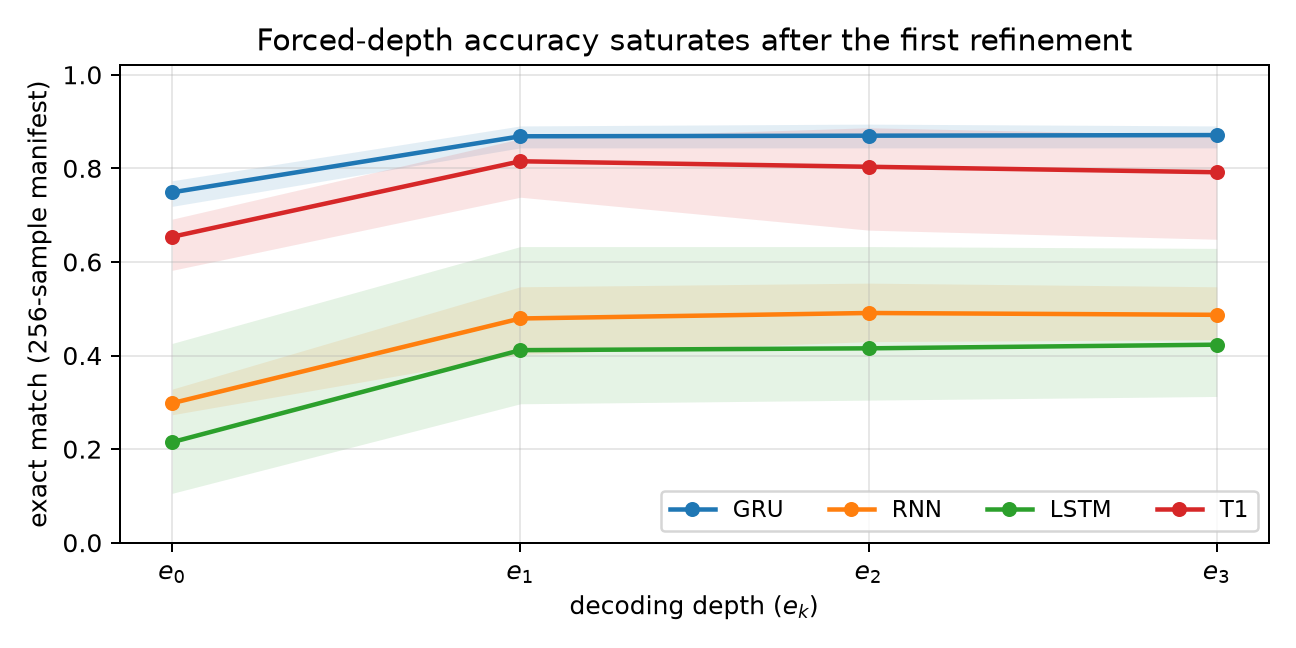
\includegraphics[width=\textwidth]{fig_depth.png}
\caption{四个架构的强制精确匹配率随深度的变化。曲线为种子均值，阴影覆盖三个种子（256 个组均衡样本）。}
\label{fig:depth}
\end{figure} \begin{table}[t]
\centering
\footnotesize
\begin{tabular}{lcccc}
\toprule
Architecture & $e_0$ & $e_1$ & $e_2$ & $e_3$ \\
\midrule
GRU & $0.749$ & $0.868$ & $0.870$ & $0.871$ \\
Vanilla RNN & $0.298$ & $0.479$ & $0.491$ & $0.487$ \\
LSTM & $0.215$ & $0.411$ & $0.415$ & $0.423$ \\
Transformer & $0.654$ & $0.815$ & $0.803$ & $0.792$ \\
\bottomrule
\end{tabular}
\caption{各深度的强制精确匹配率，每个架构对三个种子取平均（256 个组均衡样本）。}
\label{tab:depth}
\end{table} 图~\ref{fig:depth} 与表~\ref{tab:depth} 给出深度带来的收益。在各架构内，强制精确匹配从 $e_0$ 到 $e_1$ 急剧上升，随后趋于平坦：GRU、Vanilla RNN 与 LSTM 上，第一次精化贡献了 $e_3$ 所达到增益的 94\%--98\%。三种子的 $e_3$ 分数为 0.879/0.844/0.891（GRU）、0.434/0.547/0.480（Vanilla RNN）、0.629/0.312/0.328（LSTM）与 0.871/0.648/0.855（Transformer）。Transformer 的准确率同样在 $e_1$ 达到峰值，但其潜状态仍在变化，这一点在第二条主线中展开。

\begin{figure}[H]
\centering
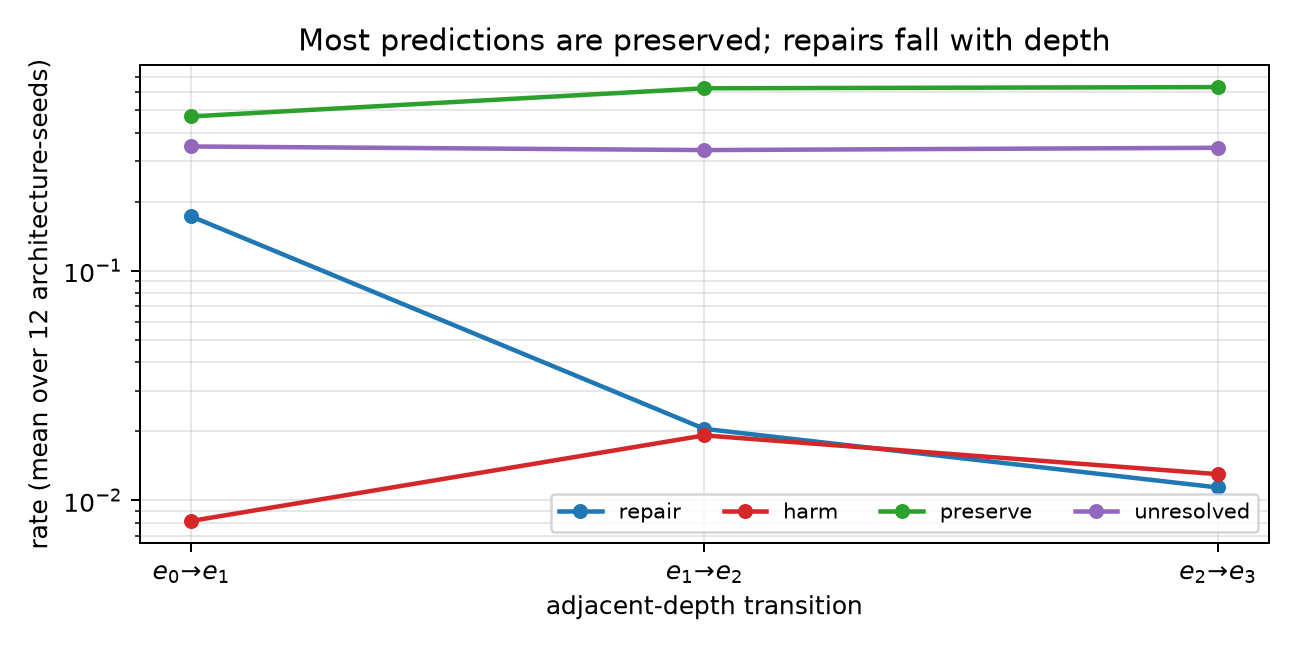
\includegraphics[width=\textwidth]{fig_transitions.png}
\caption{相邻深度之间的预测转移率，跨 12 个架构—种子取平均。}
\label{fig:transitions}
\end{figure} 相邻深度的转移解释了早期增益的来源。修复集中在第一次精化：跨 12 个架构—种子的均值从 $e_0\!\to\!e_1$ 的 0.173 降至后续的 0.021 与 0.011，保持预测从 0.471 升至 0.632。损害平均低于 0.02，但 Transformer 在 $e_1\!\to\!e_2$ 达到 0.043，因此继续精化并非普遍安全。未解决预测始终在 0.35 左右，在 LSTM 上达到 0.59，这部分输入原则上能从额外计算中获益，实际没有。

\begin{table}[t]
\centering
\footnotesize
\setlength{\tabcolsep}{1.2pt}
\resizebox{\linewidth}{!}{%
\begin{tabular}{@{}llcccccl@{}}
\toprule
架构 & 种子 & 强制 $e_3$ & 停算 & $\Delta$EM & 95\% CI & $N_{\mathrm{cell}}$ & NI \\ \midrule
GRU & $s_0$ & $0.879$ & $0.879$ & $+0.00$ & $[0.00,0.00]$ & 0.266 & \checkmark \\
GRU & $s_1$ & $0.844$ & $0.844$ & $+0.00$ & $[0.00,0.00]$ & 0.268 & \checkmark \\
GRU & $s_2$ & $0.891$ & $0.891$ & $+0.00$ & $[0.00,0.00]$ & 0.267 & \checkmark \\
Vanilla RNN & $s_0$ & $0.434$ & $0.438$ & $+0.39$ & $[0.00,1.17]$ & 0.317 & \checkmark \\
Vanilla RNN & $s_1$ & $0.547$ & $0.551$ & $+0.39$ & $[0.00,1.17]$ & 0.324 & \checkmark \\
Vanilla RNN & $s_2$ & $0.480$ & $0.461$ & $-1.95$ & $[-3.91,-0.39]$ & 0.322 & $\times$ \\
LSTM & $s_0$ & $0.629$ & $0.629$ & $+0.00$ & $[0.00,0.00]$ & 0.302 & \checkmark \\
LSTM & $s_1$ & $0.312$ & $0.312$ & $+0.00$ & $[0.00,0.00]$ & 0.320 & \checkmark \\
LSTM & $s_2$ & $0.328$ & $0.328$ & $+0.00$ & $[0.00,0.00]$ & 0.324 & \checkmark \\
Transformer & $s_0$ & $0.871$ & $0.848$ & $-2.34$ & $[-5.47,0.78]$ & 0.260 & $\ ?$ \\
Transformer & $s_1$ & $0.648$ & $0.703$ & $+5.47$ & $[1.17,10.16]$ & 0.262 & \checkmark \\
Transformer & $s_2$ & $0.855$ & $0.809$ & $-4.69$ & $[-7.81,-1.95]$ & 0.267 & $\times$ \\
\bottomrule
\end{tabular}%
}
\caption{256 样本上的阈值停算。$\Delta$EM 相对强制 $e_3$；NI 按 LCB$_{95}\geq-0.5$pp。$N_{\mathrm{cell}}$ 为停算与强制 $e_3$ 的调用比。$\times$：显著变差；$?$：不确定。九非劣、两显著负、一不确定。}
\label{tab:halt12}
\end{table} 表~\ref{tab:halt12} 是共享 256 样本上的准确率—计算量主要证据。该规则在 12 个架构—种子中的 9 个上非劣或更优，2 个显著更差（Vanilla RNN $s_2$：$-1.95$pp，95\% CI $[-3.91,-0.39]$；Transformer $s_2$：$-4.69$pp，$[-7.81,-1.95]$），1 个不确定（Transformer $s_0$：$-2.34$pp，$[-5.47,0.78]$）。$N_{\mathrm{cell}}$ 比例为 0.260--0.324，即执行的解码与精化调用减少 67\%--74\%，但这并不意味着每个种子都能无损停算。规则在深度一后已饱和处安全，在后续深度仍有收益时有害。非劣效由预注册下界 LCB$_{95}\geq-0.5$pp 决定，而非点估计。

调用减少在执行层面得到验证。在 GRU、Vanilla RNN 与 LSTM 上，强制 $e_0$、$e_1$、$e_3$ 与阈值规则的 12 种设置均与参考解码器完全一致（$12/12$），前向钩子的行数在全部 24 项核对中满足两个恒等式。强制 $e_0$ 下，带插桩的解码器在全部 52{,}458 个生成词元上触发零次精化调用。\begin{table}[t]
\centering
\begin{tabular}{lcccc}
\toprule
Model & $b{=}1$ & $b{=}4$ & $b{=}8$ & $b{=}32$ \\
\midrule
GRU & 0.439 & 0.440 & 0.484 & 0.577 \\
Vanilla RNN & 0.452 & 0.468 & 0.555 & 0.640 \\
LSTM & 0.430 & 0.471 & 0.538 & 0.611 \\
\bottomrule
\end{tabular}
\caption{active-subset 执行器的停算与强制 $e_3$ 中位墙钟时间比；两线程、2 次预热、10 次交错测试；$b{=}1$ 用 16 个样本，$b{=}4/8/32$ 用 64 个。逐样本 Transformer 执行器（0.297）为独立测量，未并入本表。}
\label{tab:wall}
\end{table} 计时使用两线程、2 次预热与 10 次交错测试，$b{=}1$ 用 16 个样本，$b{=}4/8/32$ 用 64 个。active-subset 执行器给出 0.430--0.640 的停算与强制 $e_3$ 之比；在 $b{=}32$ 时节省约 36\%--42\%，因为基步、注意力、输出投影、门控与每步 Python 工作由两侧共同承担，且不计入 $N_{\mathrm{cell}}$。另有一个逐样本 Transformer 执行器在相同 16 个样本上给出 0.297；这是不同的测量协议，不与 active-subset 比例合并。

\textbf{跨架构潜状态动力学。} \begin{figure}[H]
\centering
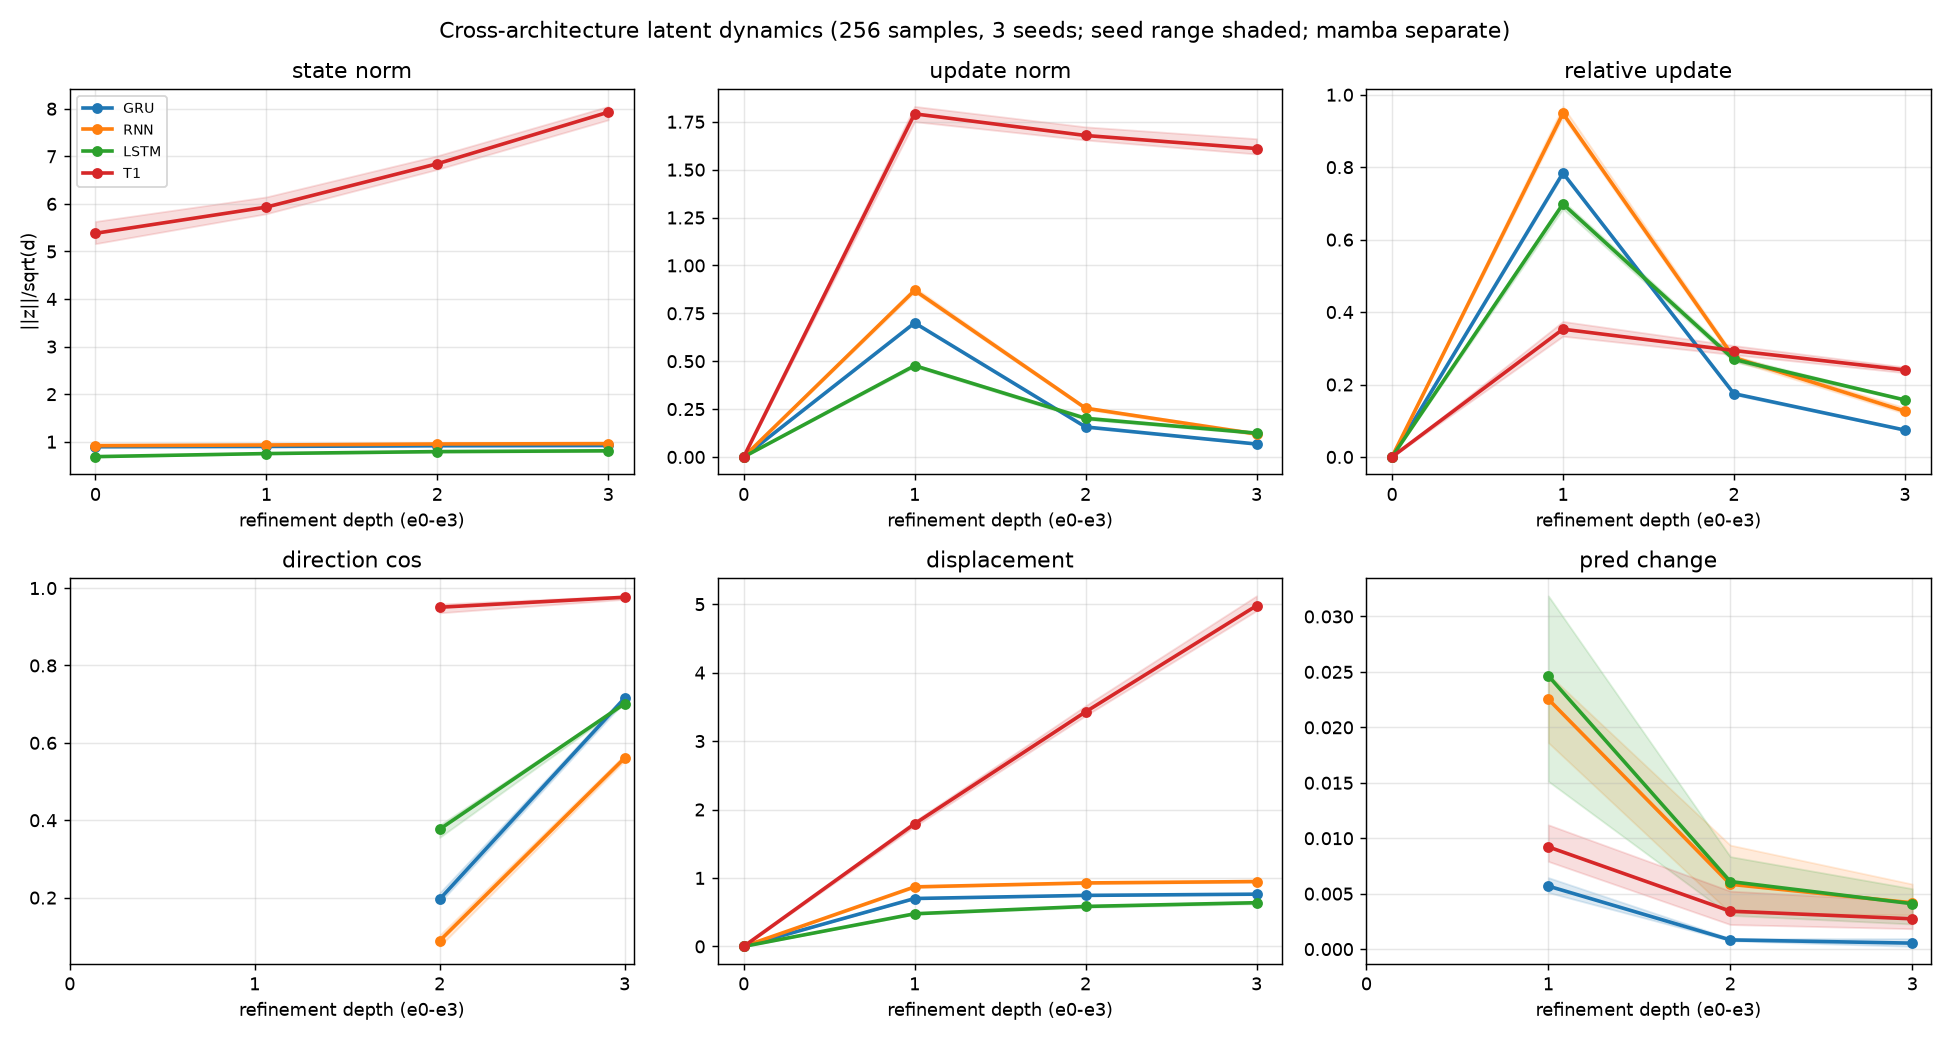
\includegraphics[width=\textwidth]{crossarch_latent_figure.png}
\caption{四个架构的六项潜状态动力学指标随深度的变化，阴影为种子范围。}
\label{fig:latcross}
\end{figure} \begin{table}[t]
\centering
\footnotesize
\resizebox{\linewidth}{!}{%
\begin{tabular}{@{}lcccc@{}}
\toprule
Arch & norm $e_0$ & upd $e_1$ & cos $e_2$ & $\Delta y$ $e_3$ \\ \midrule
GRU & 0.90 $[0.90,0.90]$ & 0.70 $[0.70,0.70]$ & 0.19 $[0.18,0.19]$ & 0.0004 $[0.0002,0.0007]$ \\
Vanilla RNN & 0.92 $[0.92,0.92]$ & 0.89 $[0.88,0.89]$ & 0.09 $[0.09,0.09]$ & 0.0059 $[0.0038,0.0082]$ \\
LSTM & 0.69 $[0.69,0.69]$ & 0.48 $[0.48,0.48]$ & 0.39 $[0.38,0.39]$ & 0.0023 $[0.0014,0.0032]$ \\
Transformer & 5.16 $[5.13,5.20]$ & 1.83 $[1.83,1.84]$ & 0.96 $[0.96,0.96]$ & 0.0020 $[0.0012,0.0030]$ \\
\bottomrule
\end{tabular}%
}
\caption{种子 0 的均值与 95\% 组簇自助区间（256 样本）。三种子的范围见图~\ref{fig:latcross}；范数为 $\lVert z_k\rVert/\sqrt d$。}
\label{tab:latstat}
\end{table} 图~\ref{fig:latcross} 与表~\ref{tab:latstat} 汇总了在 256 个组均衡样本上以自由运行贪心解码记录的六项轨迹指标；词元级数值先在样本内平均，再做 20{,}000 次组簇自助。两类状态分离。有界门控态（GRU、Vanilla RNN、LSTM 隐状态）的归一化范数在 0.68--0.96 之间，更新随深度收缩；第一次精化承载其总位移的 75\%--92\%。无界累积态（LSTM 细胞状态与 Transformer）处于 5 到 8 的尺度并持续变化。LSTM 的隐状态与细胞状态分开报告，因为二者行为不同。差别最大的是方向：在 $e_2$，有界组的更新余弦为 0.07--0.39，Transformer 达到 0.95，更新持续共线且范数增长。预测变化率在所有架构中都随深度下降。这些是模型内描述，不是跨架构排名；绝对范数在模型之间不可比，注意力类型与参数量同时变化，单种子 Mamba-1-Tiny 探针不进入四架构统计：其 256 样本组均衡重评 给出 $e_3=0.246$ 低于 0.30 门槛，其 64 样本潜状态轨迹仅作描述。

\textbf{进化式步长控制与迁移。} \begin{table}[t]
\centering
\footnotesize
\begin{tabular}{@{}lcccc@{}}
\toprule
Algorithm & Mean (pp) & Median (pp) & Std (pp) & Win \\ \midrule
RS & $+0.64$ & $+0.52$ & 0.63 & 67\% \\
GA & $+0.81$ & $+0.52$ & 0.64 & 89\% \\
MGA & $+0.46$ & $+0.52$ & 0.17 & 89\% \\
DE & $+0.81$ & $+0.52$ & 0.53 & 89\% \\
sepCMA & $+0.41$ & $+0.52$ & 0.35 & 67\% \\
\bottomrule
\end{tabular}
\caption{45 次搜索中的五种优化器（3 模型种子 × 5 算法 × 3 优化器种子，各 336 次评估）。增益为相对 $\alpha\equiv1$ 基线的 pp，192 样本内层子集，一个样本为 $0.52$pp；MGA 作为独立算法报告。}
\label{tab:opt5}
\end{table} \begin{figure}[H]
\centering
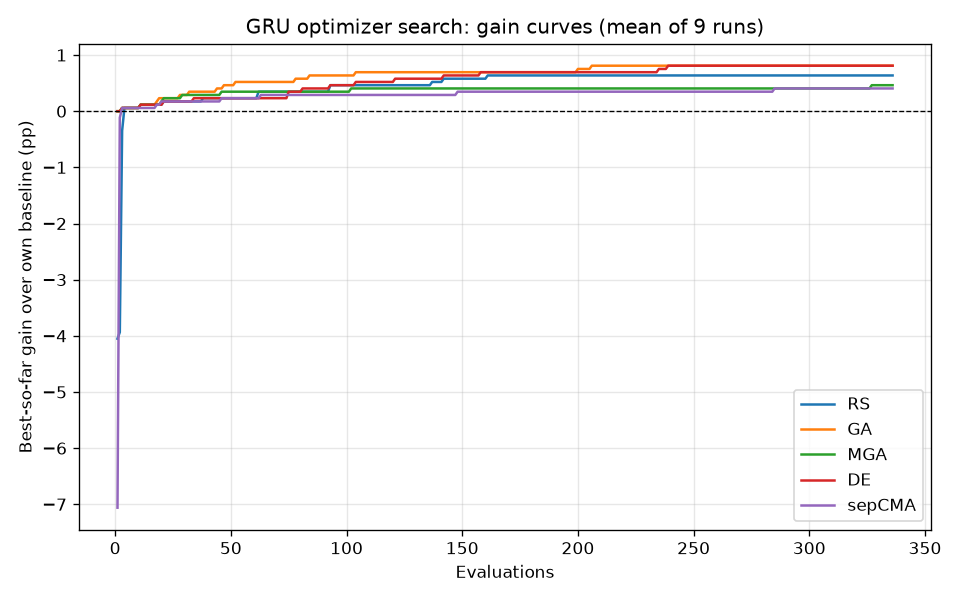
\includegraphics[width=\textwidth]{optimizer_curves.png}
\caption{每次搜索相对自身基线的最佳至当前增益（每种算法九次运行的均值）。}
\label{fig:optcurves}
\end{figure} 表~\ref{tab:opt5} 汇总全部 45 次搜索：3 模型种子 × 5 算法 × 3 优化器种子，每次 336 次评估。五种算法 RS、GA、MGA、DE 与 sep-CMA-ES 的中位增益相同，均为 $+0.52$pp，正好是 192 样本内层子集中的一个样本；GA 与 DE 均值为 $+0.81$pp，MGA 为 $+0.46$pp，RS 为 $+0.64$pp，sep-CMA-ES 为 $+0.41$pp，胜率 67\%--89\%。跨模型种子基线 EM 相差 2.4pp，是搜索效应的数倍，单次 $+2.08$pp 运行是异常点。随机搜索具有竞争力，没有优化器稳定胜出；三个优化器种子不足以支持算法排名。192 样本子集把任何增益量化到约 0.52pp，这限制了可得出的结论。图~\ref{fig:optcurves} 给出每次运行相对自身基线的最佳至当前增益。

\begin{table}[t]
\centering
\footnotesize
\begin{tabular}{@{}llccl@{}}
\toprule
Seed & Best & Outer $\Delta$EM & 95\% CI (pp) & NI \\ \midrule
$s_0$ & DE & $+0.000$ & $[-0.519,+0.527]$ & $\times$ \\
$s_1$ & GA & $-0.469$ & $[-1.357,+0.000]$ & $\times$ \\
$s_2$ & DE & $+0.000$ & $[-0.469,+0.538]$ & \checkmark \\
\bottomrule
\end{tabular}
\caption{三个 GRU 步长策略的外层折确认（每种子 $n=640$）。仅种子 2 满足非劣效界；种子 0 以 0.019pp 之差未过界（LCB $-0.519$pp）。}
\label{tab:alpha_confirm}
\end{table} 在内层子集上选择并在外层评估前冻结策略，得到表~\ref{tab:alpha_confirm} 的确认结果。在 640 样本外层折上只有种子 2 满足非劣效界；种子 0 以 0.019pp 之差未过界（LCB $-0.519$pp），种子 1 明显失败。因此内层增益并未成为可靠的外层增益。\begin{table}[t]
\centering
\footnotesize
\setlength{\tabcolsep}{2pt}
\begin{tabular}{@{}lccl@{}}
\toprule
Target & Seed & $\Delta$ (pp) & 95\% CI / verdict \\
\midrule
Vanilla RNN & 0 & $-0.39$ & $[-1.17,0.00]$ inconclusive \\
Vanilla RNN & 1 & $+1.17$ & $[-0.39,3.12]$ non-inferior \\
Vanilla RNN & 2 & $+0.39$ & $[0.00,1.17]$ non-inferior \\
LSTM & 0 & $-0.78$ & $[-1.95,0.00]$ inconclusive \\
LSTM & 1 & $+0.78$ & $[-0.78,2.34]$ inconclusive \\
LSTM & 2 & $-0.39$ & $[-1.17,0.00]$ inconclusive \\
Transformer & 0 & $+2.34$ & $[0.00,4.69]$ non-inferior \\
Transformer & 1 & $+3.52$ & $[0.39,6.64]$ non-inferior \\
Transformer & 2 & $-0.39$ & $[-2.73,1.95]$ inconclusive \\
\bottomrule
\end{tabular}
\caption{冻结的 GRU-s0 步长策略：各种子相对强制 $e_3$ 的 EM 差（pp）。}
\label{tab:trans}
\end{table} 把在 GRU 种子 0 上选出并冻结的 GA 策略在没有目标架构搜索的情况下原样用于 Vanilla RNN、LSTM 与 Transformer，得到表~\ref{tab:trans} 的九个逐种子结果：四个非劣、五个不确定、无显著变差。这是同一协议下的部分迁移，不是普适的跨架构能力，且架构种子数不足以排名。\begin{table}[H]
\centering
\footnotesize
\setlength{\tabcolsep}{2.5pt}
\resizebox{\linewidth}{!}{%
\begin{tabular}{llcccccc}
\toprule
种子 / 基准 & 基准 EM & 阈值 EM & $\Delta$EM (pp) & 95\% CI (pp) & 比率 & 非劣效 \\
\midrule
$s_0$ / $e_3$ & 95.53 & 95.43 & $-0.10$ & $[-0.23, 0.00]$ & 0.2572 & \checkmark \\
$s_1$ / $e_3$ & 97.13 & 97.07 & $-0.07$ & $[-0.17, 0.00]$ & 0.2573 & \checkmark \\
$s_2$ / $e_1$ & 96.77 & 96.97 & $+0.20$ & $[-0.10, +0.51]$ & 0.5182 & \checkmark \\
\bottomrule
\end{tabular}%
}
\caption{\textbf{在未触碰数据上的一次性确认。} 官方 COGS 开发集（$n{=}3{,}000$；组聚类配对自助，20{,}000 次重采样），用冻结的预注册阈值与各种子冻结的最佳固定深度只评估一次。计算量比率与留出折的数值（0.2575 / 0.2570 / 0.5212）在种子0--1上到第三位小数一致，种子2相差0.003（相对0.6\%），因此被执行调用层面的节省本身在划分之间以不足百分之一的幅度迁移。}
\label{tab:devconfirm}
\end{table} 最后，冻结阈值规则在未触碰的 3{,}000 样本 COGS 开发集上只评估一次（表~\ref{tab:devconfirm}）；执行调用比在两个种子上与留出值相差不超过 0.003，在第三个种子上相差 0.003。综合来看，搜索带来的是微小且受分辨率限制的增益，冻结的更新策略只在部分目标上迁移。

\section{结论}
\label{sec:conclusion}

递归的收益并不均匀分布在各深度。若干种子在第一次精化后已经稳定，后续步骤改动很小；因果阈值在这些步骤上停算，多数架构种子并未损失准确率。同一固定阈值仍让两个种子（Vanilla RNN $s_2$、Transformer $s_2$）损失准确率，能省多少因而取决于各深度曲线在何处饱和。

潜状态轨迹为这一分界提供了机制层面的刻画。有界门控态在第一次精化后收缩更新，无界累积态则沿一致方向持续累加。首次精化后的饱和属于有界态，并非递归模型的普遍规律；绝对状态范数也不能在不同架构间当作排名来读。

进化搜索对固定步长的改动很小。45 次等预算搜索的增益中位数只有 1 个样本（内层子集共 192 个），没有哪个优化器稳定胜出。选出的步长策略只在三个种子中的一个上通过外层确认；同一冻结策略在 9 次迁移中有 4 次非劣。这些增益没有变成可靠的跨架构改进，我们把这一差距看成方法本身的局限，而不是实现细节。

TRACER 把三件事放在一起：追踪预测与状态，判断是否需要再算一步，检验调整后的更新能走多远。更深的层数并不总是更高的准确率；知道额外步骤何时有用、控制规则换到新模型上是否仍成立，与增加深度本身同样重要。三条主线围绕同一件事展开：追踪递归状态以理解深度何时有用，停算以避免冗余精化，进化更新策略以检验它的适用边界，并记录每条规则在哪里成立、在哪里失效。

\section*{局限性}
有限的计算资源使模型规模较小，架构与种子数量也不多。实验只覆盖 COGS 一个语义解析数据集，观察到的模式不应直接推及大语言模型或更广的推理任务。四个架构在注意力类型与参数量上也不相同，因此这些比较描述的是同一任务下的行为变体，而不是对循环单元的受控消融。实验在 CPU 上以固定两线程设置完成，墙钟数字只描述这一环境，不代表大规模 GPU 服务或深得多的递归。至于潜状态动力学与控制规则在这些设置下是否仍然成立，目前还没有答案。

\bibliographystyle{acl_natbib}
\bibliography{references}

\end{document}
